\documentclass[journal]{IEEEtran}
\IEEEoverridecommandlockouts

\renewcommand\IEEEkeywordsname{Palabras Clave}

\usepackage[spanish]{babel}
\usepackage[utf8x]{inputenc}
\usepackage{cite}
\usepackage{amsmath,amssymb,amsfonts}
\usepackage{algorithmic}
\usepackage{graphicx}
\usepackage{textcomp}
\usepackage{xcolor}
\usepackage{fancyhdr}
\usepackage{listings}
\usepackage{float}
\usepackage{blindtext}
\usepackage{newtxmath}
\usepackage{wrapfig}
\usepackage{mathtools}

\lstdefinestyle{code}{%
backgroundcolor=\color{gray!5},
basicstyle=\ttfamily\small,
commentstyle=\color{green!60!black},
keywordstyle=\color{magenta},
stringstyle=\color{blue!50!red},
showstringspaces=false,
%captionpos=b,
numbers=left,
numberstyle=\footnotesize\color{gray},
numbersep=8pt,
%stepnumber=2,
tabsize=2,
%frame=L,
%framerule=1pt,
%rulecolor=\color{red},
breaklines=true,
}

\def\BibTeX{{\rm B\kern-.05em{\sc i\kern-.025em b}\kern-.08em
    T\kern-.1667em\lower.7ex\hbox{E}\kern-.125emX}}


\graphicspath{ {../Imagenes/} }

\begin{document}
    \title{Simulador Dinámico de un Exoesqueleto de 6GdL\\
    \small{Reporte de Medio Término}}

    \author{\IEEEauthorblockN{García-Álvarez Gregorio E. , Luna-Macías Antonio J. , Tevera-Ruiz Alejandro\\}
    \IEEEauthorblockA{\textit{Departamento: Roobótica y Manufactura Avanzada} \\
    \textit{Centro de Investigación y de Estudios Avanzados (CINVESTAV)}}
    }

    \maketitle

    \begin{abstract}
        El presente documento describe el desarrollo cinemático y dinámico que simula un exoesqueleto
        con 6 grados de libertad (GDL).
        \noindent El diseño está enfocado para utilizarse en el dedo índice, sin embargo debido a que
        este trabajo aún no incorpora otras cadenas cinemáticas, como el diseño original presentado en
        el trabajo: "HEXOTRAC"[1], esto implica que el propio, se pueda utilizar adecuadamente en
        cualquier dedo a excepción del pulgar. 
        \noindent Una de las características que tendrá el exoesqueleto presentado, será que el dedal
        distal, tendrá capacidades hápticas y estará actuado en todos sus grados de libertad,
        sin embargo por el momento, no es el alcance concerniente a este documento.         
    \end{abstract}

    \begin{IEEEkeywords}
    Simulador, Exoesqueleto, GRyMA
    \end{IEEEkeywords}

    \section{Introducción}

    \blindtext[0]

    \section{Descripción Metodológica}

    El diseño del dedo exoesqueleto con 6 GDL se muestra en la Figura \ref{fig:Diseno3D} en su 
posición inicial de "CASA" y está constituido por una cadena cinemática de 7 eslabones, que 
están todos conectados entre sí por articulaciones revolutas. El software que se utilizó para 
generar el diseño en 3D, fue solidworks porque tiene varias herramientas que ayudaron en el 
desarrollo matemático, así como su versatilidad para enlazarse con matlab, software con el que 
se programaron los cálculos.  

\begin{figure}[H]
    \centering
    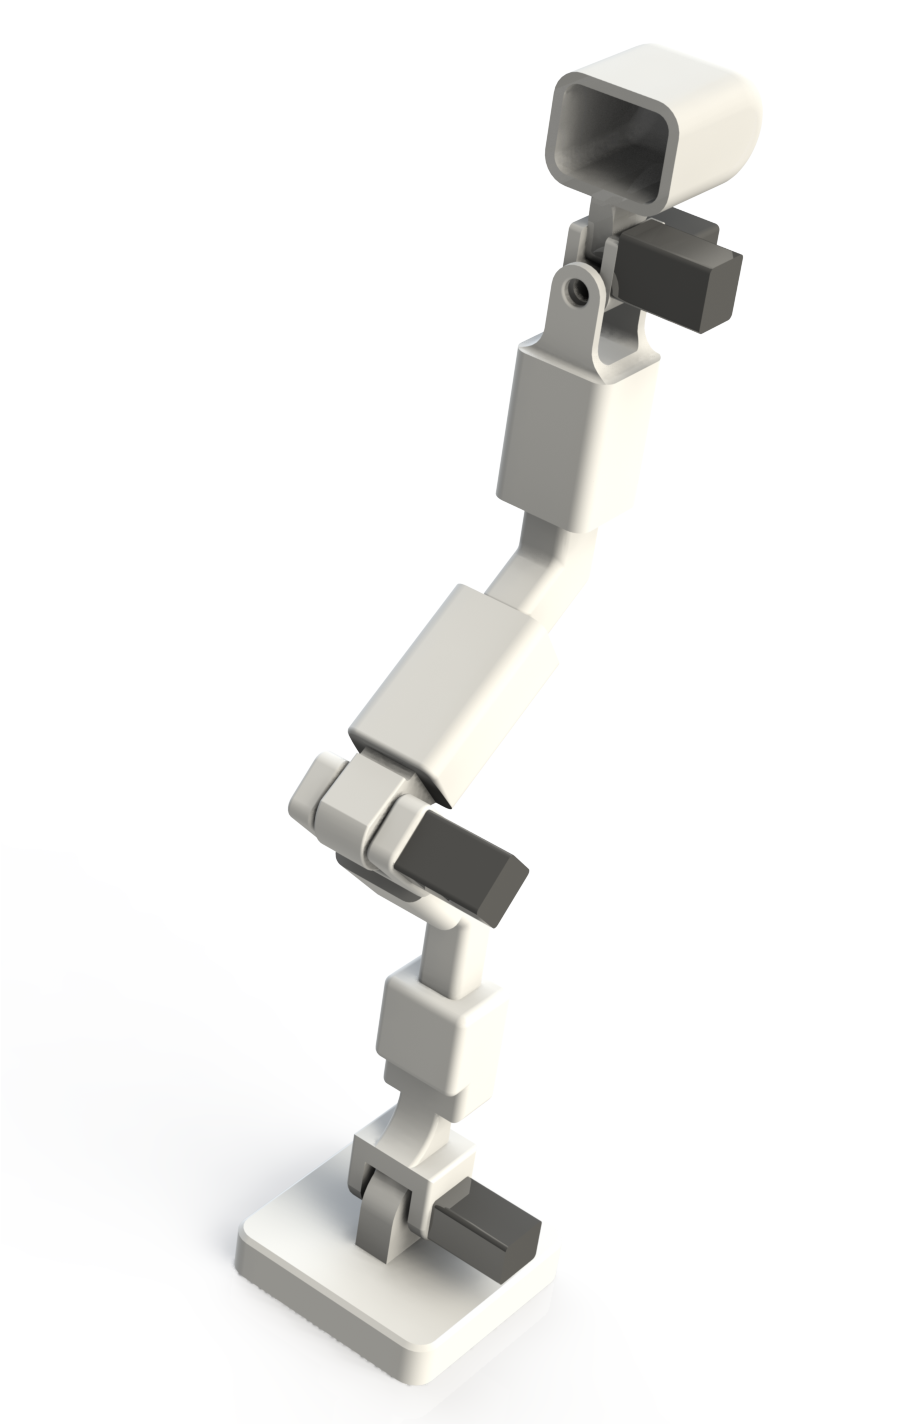
\includegraphics[scale=0.2]{Dedo Vist Isometrica.png} 
    \caption{Diseño 3D}
    \label{fig:Diseno3D}
\end{figure}

La disposición de las articulaciones que se muestran en la Figura \ref{fig:EsqArtOri}, fueron las 
planteadas en el trabajo HEXOTRAC: A highly Under-Actuated Hand Exoskeleton for Finger Tracking 
and Force Feedback (REFERENCIA).

\begin{figure} [H]
    \centering
    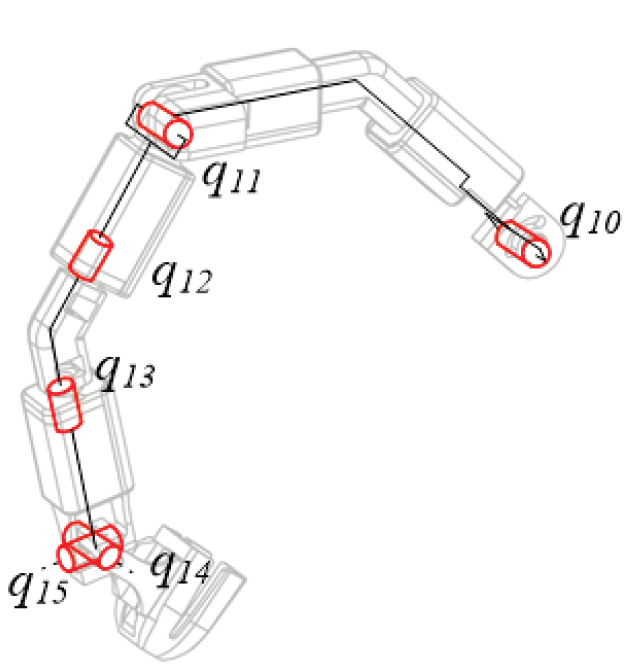
\includegraphics[scale=0.4]{EsquemaArticulaciones.png} 
    \caption{Esquema de las Articulaciones Original}
    \label{fig:EsqArtOri}
\end{figure}

Sin embargo por el equipo propuso una modificación y se agregó un eslabón más, de esta manera 
se evita que la articulación revoluta  $q_{14}$ y  $q_{15}$ estuvieran fusionadas, como se 
visualiza en la Figura \ref{fig:EsqArtOri}. El dibujo posicionado con una perspectiva lateral 
derecha, que se visualiza en la Figura \ref{fig:ExoPara} proporciona una imagen con dimensiones 
parametrizadas, mismas que se plasman en la siguiente tabla: 

\begin{table}[!ht] %[H]
    \centering
    \begin{center}
        \begin{tabular}{ccc}
        Parámetros & [m] \\
        \hline \hline 
        L1 & 0.03235525  \\ 
        L2 & 0.10513390  \\
        L3 & 0.02462267  \\
        L4 & 0.02228474  \\
        L5 & 0.04334075  \\
        L6 & 0.00600000  \\
        L7 & 0.01999013  \\
        L8 & 0.02565247  \\
        L9 & 0.01273194  \\
        L10 & 0.03641522 \\
        \end{tabular}
    \end{center}
\end{table}

Cabe destacar que el ángulo $\alpha$ que aparece en la imagen \ref{fig:ExoPara} es 
$\alpha$ = 59.26721315 [rad]. En la misma figura \ref{fig:ExoPara} se aprecia la asignación 
de referenciales $\Sigma_0$, $\Sigma_1$, $\Sigma_2$, $\Sigma_3$, $\Sigma_4$, $\Sigma_5$,  
$\Sigma_6$ y $\Sigma_7$. Los marcos inerciales propuestos a cada GdL se colocaron utilizando 
la convención GRyMA, manteniendo la dirección positiva de la mano derecha.

También se asignaron materiales, proponiendo para los eslabones un polímero termoplástico de 
nombre "acrilonitrilo butadieno estreno" también conocido como filamento ABS, utilizado por 
impresoras 3D, pensando que en un futuro próximo podamos imprimir el modelo y así experimentar 
con el en un entorno real. En el caso del dedal, se seleccionó un polímero artificial que 
pertenece al grupo de las poliamidas, llamado comunmente "Nylon", pues creemos que para cuidar 
la comodidad del usuario, al ingresar su dedo, el material no debe ser tan rígido y el nylon 
permite un equilibrio entre la suavidad y al mismo tiempo que no sea deformable.

Finalmente los motores propuestos son de micro Metal LP con reductora de 50:1, de corriente 
continua, con dimensiones de 24 x 10 x 12 mm y 10 gramos de peso. 

Al proponer materiales específicos, conocer sus dimensiones e incorporar las masas del motor 
pololu, se puede conocer el peso total del exoesqueleto, así como sus centros de masa 
(REFERENCIA TABLA 1 ANEXOS ) y los tensores de inercia de cada eslabón 
(REFERENCIA MATRICES EN ANEXOS), esta información se encuentra descrita en la sección de ANEXO  

\begin{figure}[H]
    \centering
    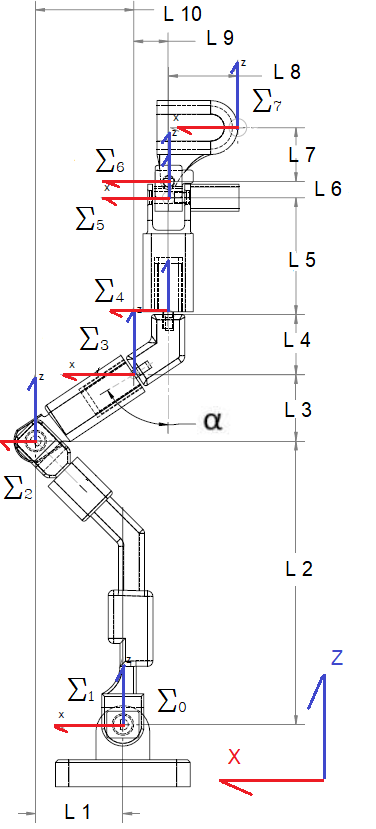
\includegraphics[scale=0.7]{ExoParametrizado.png}
    \caption{Esquema de las Articulaciones Utilizado}
    \label{fig:ExoPara}
\end{figure}

Conocer la cantidad de grados de libertar que tiene el exoesqueleto, nos servirá para identificar 
la versatilidad del movimiento que se podrá ejercer. Existen 3 clasificaciones [2]:

\begin{itemize}
    \item Menos de 6 GDL.  si el robot está diseñado para moverse en un espacio tridimensional, presentará  limitaciones su movimiento. 
    \item Exactamente 6 GDL. Se podrá mover de manera independiente en cada uno de los seis parámetros que conforman el espacio de trabajo tridimensional.
    \item Más de 6 GDL. Si un robot tiene más actuadores que los parámetros del espacio, implica que está sobre actuado.
\end{itemize}


    \subsection{Cinemática directa}
    \subsubsection{Transformaciones homogéneas}
        \noindent De manera general, se explica una matriz de transformación homogénea como una
        matriz que permite expresar un punto especificado en coordenadas de
        un marco referencial con respecto a las coordenadas de otro marco 
        referencial, esto a partir de la aplicación de una rotación pura, 
        una traslación pura, o una combinación de ambas sobre el marco referencial
        inicial.

        De esta forma, se explica en \cite{3DMotion} que para cadenas cinemáticas abiertas, 
        donde el movimiento se encuentra restringido a una sola dirección, la 
        transformación homogénea desde el referencial padre hacia cualquier referencial 
        local se define únicamente por las coordenadas generalizadas escalares 
        correspondientes, definido de la siguiente manera.
        \begin{equation*} 
            A_i(q_i) \triangleq A^i_{pi}(q_i) =
            \begin{bmatrix}
                R^i_{pi}(q_i) & d^i_{pi}\\
                0 & 1
            \end{bmatrix}
            \in SE(3)
        \end{equation*}
        Donde \emph{i} representa el marco referencial del cuerpo
        correspondiente, y \emph{pi} el marco referencial padre del 
        referencial \emph{i}.

        A partir de esta definición, se afirma que la transformación homogénea representa
        el movimiento rígido de un marco referencial dado con respecto a otro, y que además 
        presenta la propiedad de la propagación del Movimiento Rígido, que de manera resumida 
        permite realizar una multiplicación entre matrices de transformación homogénea de 
        marcos referenciales consecutivos, de tal manera que la matriz resultante representa 
        la transformación entre el primer y el último marco referencial, expresándose de la 
        siguiente manera.
        \begin{equation}
            A^i_0(q) =  A^{pi}_0(q_1,...,q_j)A_i(q_i)
            \label{eq:CD}
        \end{equation}

    \subsubsection{Asignación de referenciales}
        \noindent Con respecto al tema de transformaciones homogéneas, se observa que un 
        aspecto clave que se debe tener delimitado en el sistema es la localización 
        y orientación de los diferentes referenciales correspondientes a cada uno de 
        los cuerpos rígidos que lo conforman. En este caso, se busca tener un marco 
        referencial asigando a cada uno de los eslabones de una cadena cinemática, con lo cual es 
        necesario un proceso de ubicación de referenciales en los diferentes 
        puntos de interés en el robot a analizar, conocido como asignación de referenciales.

        Como se explica en \cite{3DMotion}, existen diferentes metodologías para la asiganción 
        de referenciales en sistemas robóticos con cadenas cinemáticas abiertas. A 
        continuación, se describirá de manera resumida el fundamento de las convenciones de 
        Denavit-Hartenberg (DH), que también aplican para su versión modificada (DHm), 
        al igual que se explicará la metodología propuesta por el Grupo de Robótica y 
        Manufactura Avanzada del CINVESTAV (GRyMA), siendo esta última la metodología 
        utilizada para la asignación de referenciales en el proyecto.

        Por un lado, se tiene que las convenciones \emph{DH} y \emph{DHm}, están conformadas 
        de algoritmos que delimitan la forma de establecer marcos de referencia en 
        cadenas cinemáticas donde los marcos consecutivos dependen únicamente de 4 parámtros, 
        en vez de 6 que sería el caso de considerar todas las posibles traslaciones y rotaciones 
        en los tres ejes \emph{[x,y,z]} del sistema coordenado. Para lograr dicha reducción de 
        parámetros, las metodologías hacen uso de 2 restricciones con respecto al movimiento de 
        un marco referencial a otro.

        \begin{itemize}
            \item El eje \emph{x} de un referencial dado debe ser perpendicular al eje \emph{z} de los marcos referenciales consecutivos.
            \item El eje \emph{x} de un referencial dado y el eje \emph{z} del referencial consecutivo deben intersectar.
        \end{itemize}

        De igual manera, se asume que el movimiento de cualquier marco de referencia con respecto 
        a su referencial padre, ya sea rotacional o prismático, debe realizarse siempre con respecto 
        al eje \emph{z} del referencial padre.

    \subsubsection{Metodología GRyMA}
        \noindent Con respecto a la metodología GRyMA, se explica en \cite{3DMotion} que el proceso de asignación 
        de referenciales inicia con delimitar cada marco referencial $\Sigma_i$ a lo largo de los ejes 
        de las articulaciones que definen cada coordenada generalizada $q_i$. Sin embargo, a 
        diferencia de las metodologías \emph{DH} y \emph{DHm}, en este caso no existe la 
        restricción de colocar el eje \emph{z} en la misma dirección que la dirección de movimiento de las 
        articulaciones, con lo cual la dirección de movimiento se define directamente con el 
        vector director extendido.
        \begin{equation*}
            \boldsymbol{\lambda}_i = (\boldsymbol{\lambda}^T_T, \boldsymbol{\lambda}^T_R)^T \in \mathbb{R}^6
        \end{equation*}
        De esta manera, cada uno de los marcos referenciales se puede colocar en la misma 
        orientación que el referencial base, con lo cual solamente resultan necesarios 3 
        parámetros de ajuste para determinar la distancia relativa entre el referencial 
        padre y cada referencial local en una posición de las coordenadas generalizadas de 
        \emph{\textbf{q} = 0}.
        \begin{equation*}
            \boldsymbol{d}_{0_i} = (d_{xi}, d_{yi}, d_{xi})
        \end{equation*}
        Con lo cual, considerando que se cumple la condición de tornillo explicada en \cite{3DMotion}, 
        $\boldsymbol{\lambda}_{T_i} \times \boldsymbol{\lambda}_{R_i} = 0$, debido a que cada coordenada generalizada 
        induce ya sea un movimiento prismático o de revoluta, pero no una combinación de ambos, 
        entonces la matriz de trasformación homogénea entre dos referenciales se 
        expresa de la siguiente manera.
        \begin{equation}
            A_i(q_i) = A_{i0} A_{iv}(q_i) = 
            \begin{bmatrix}
                e^{[\boldsymbol{\lambda}_{R_i}\times]q_i} & \boldsymbol{d}_{0_i} + \boldsymbol{\lambda}_{Ti}q_i\\
                0 & 1
            \end{bmatrix}
            \label{eq:TH_GRYMA}
        \end{equation}
        Considerando que el \emph{Operador Producto Cruz} 
        [\textbf{a}$\times$] representa el producto cruz vectorial como una expresión 
        de una matriz simétrica de la siguiente forma.
        \begin{equation*}
            [\mathbf{a}\times] = 
            \begin{bmatrix}
                0 & -a_z & a_y\\
                a_z & 0 & -a_z\\
                -a_y & a_x & 0
            \end{bmatrix}
            \in \mathbb{R}^{3x3}
        \end{equation*}
        Así, si todos los posibles movimientos se encuentran alineados con alguno de los 
        ejes principales de cada marco referencial, el vector director cinemático $\boldsymbol{\lambda}_i$ 
        puede ser codificado con un parámetro escalar único $\Theta$, incluyendo el caso constante, 
        es decir el caso en el que no existe un movimiento variable en el tiempo.
        \begin{table}[H]
            \caption{Códigos de movimiento GRyMA}
            \centering
                \begin{center}
                    \begin{tabular}{cccccccc}
                        $\Theta_i$ & 0 & 1 & 2 & 3 & 4 & 5 & 6\\
                        \hline \hline 
                        $\boldsymbol{\lambda}_{T_i}$ & 0 & 1 & 0 & 0 & 0 & 0 & 0\\ 
                        $\boldsymbol{\lambda}_{T_i}$ & 0 & 0 & 1 & 0 & 0 & 0 & 0\\
                        $\boldsymbol{\lambda}_{T_i}$ & 0 & 0 & 0 & 1 & 0 & 0 & 0\\
                        \hline 
                        $\boldsymbol{\lambda}_{R_i}$ & 0 & 0 & 0 & 0 & 1 & 0 & 0\\
                        $\boldsymbol{\lambda}_{R_i}$ & 0 & 0 & 0 & 0 & 0 & 1 & 0\\
                        $\boldsymbol{\lambda}_{R_i}$ & 0 & 0 & 0 & 0 & 0 & 0 & 1\\
                        \hline 
                        $R_{i}$ & $I_3$ & $I_3$ & $I_3$ & $I_3$ & $R_{x}(qi)$ & $R_{y}(qi)$ & $R_{z}(qi)$\\
                    \end{tabular}
                \end{center}   
        \end{table}
        Con lo cual, la metodología GRyMA haría uso de 4 parámetros básicos constantes 
        para cada relación padre/hijo entre referenciales: $d_{x_1}, d_{y_1}, d_{z_1}$ 
        y $\Theta_i$.

        De otra manera, cada vector director de traslación y rotación puede ser parametrizado 
        con un par de elevación-azimuth $(\alpha_i,\beta_i)$ de la siguiente manera, 
        aumentando el número de parámetros requeridos en 2. 
        \begin{table}[H]
            \caption{Códigos generales GRyMA}
            \label{tb:generales_gryma}
            \centering
            \begin{center}
                \begin{tabular}{ccc}
                    $\Theta_i$ & 7 & 8\\
                    \hline \hline 
                    $\boldsymbol{\lambda}_{T_i}$ & $\cos{(\alpha_i)}\sin{(\beta_i)}$ & 0\\ 
                    $\boldsymbol{\lambda}_{T_i}$ & $\sin{(\alpha_i)}\sin{(\beta_i)}$ & 0\\
                    $\boldsymbol{\lambda}_{T_i}$ & $\cos{(\beta_i)}$ & 0\\
                    \hline 
                    $\boldsymbol{\lambda}_{R_i}$ & 0 & $\cos{(\alpha_i)}\sin{(\beta_i)}$\\
                    $\boldsymbol{\lambda}_{R_i}$ & 0 & $\sin{(\alpha_i)}\sin{(\beta_i)}$\\
                    $\boldsymbol{\lambda}_{R_i}$ & 0 & $\cos{(\beta_i)}$\\
                    \hline 
                    $R_{i}$ & $I_3$ & $R_{\boldsymbol{\lambda}_{R_i}}$(qi)\\ 
                \end{tabular}
            \end{center}
        \end{table}
    \subsubsection{Jacobiano geométrico}
        \noindent Se explica en \cite{3DMotion} que el Jacobiano geométrico de un marco referencial 
        específico es el operador lineal que permite mapear las velocidades generalizadas 
        $\textbf{\dot{q}}$ a los valores del \emph{twist} $\mathcal{V}_i$, el cual es el vector que 
        contiene la velocidad lineal y angular de un marco referencial, y se define de la 
        siguiente manera. 
        \begin{equation*}
            \mathcal{V}  \triangleq 
            \begin{pmatrix}
                v \\
                \omega
            \end{pmatrix}
            \in \mathcal{M} \subset \mathbb{R}^6
        \end{equation*}
        Considerando a $\mathcal{M}$ como el espacio de movimiento del robot. Con lo cual, al ser relacionado con el Jacobiano geométrico, se obtiene la siguiente 
        igualdad.
        \begin{equation*}
            \mathcal{V} = J_i(\boldsymbol{q})\boldsymbol{\dot{q}}
        \end{equation*}
        De esta manera, se observa que al ser el \emph{twist} un vector que puede ser expresado 
        en las coordenadas de cualquier marco referencial, entonces también es posible expresar 
        el Jacobiano geométrico de diferentes formas. En este caso surgen las siguientes expresiones 
        para la representación del Jacobiano en coordenadas inerciales y locales.
        \begin{align*}
            \mathcal{V}^{(0)}_i = \prescript{0}{}J_i(\boldsymbol{q})\boldsymbol{\dot{q}} \\
            \mathcal{V}^{(i)}_i = \prescript{i}{}J_i(\boldsymbol{q})\boldsymbol{\dot{q}}
        \end{align*} 
        Así mismo, debido a la definición que tiene el vector \emph{twist},  
        el Jacobiano geométrico puede ser descompuesto en sus elementos referentes a velocidad 
        lineal y velocidad angular de la siguiente manera.
        \begin{equation*}
            \prescript{j}{}J_i(\boldsymbol{q}) = 
            \begin{bmatrix}
                \prescript{j}{}J_{v_i}(\boldsymbol{q}) \\
                \prescript{j}{}J_{\omega_i}(\boldsymbol{q})
            \end{bmatrix}
        \end{equation*}
        De tal manera que se tienen las siguientes equivalencias para la velocidad lineal y angular del 
        referencial local analizado.
        \begin{align*}
            v^{(j)}_i = \prescript{j}{}J_{v_i}(\boldsymbol{q})\dot{\boldsymbol{q}} \\
            \omega^{(j)}_i = \prescript{j}{}J_{\omega_i}(\boldsymbol{q})\boldsymbol{\dot{q}}
        \end{align*}
        Cabe mencionar que los componentes de velocidad del Jacobiano pueden ser expresados 
        con respecto al referencial inercial, solamente es necesario hacer la multiplicación 
        por la matriz de transformación homogénea respectiva del referencial inercial al referencial 
        correspondiente del Jacobiano local.

    \subsubsection{Jacobiano geométrico de velocidad lineal}
        \noindent Como primer punto se explica en \cite{3DMotion} que el Jacobiano de velocidad lineal 
        en una cadena serial, puede ser expresado de la siguiente manera.
        \begin{equation}
            \prescript{0}{}J_{Vi}(\boldsymbol{q}) = 
            \left[{[\prescript{0}{}J_{V_i}]}_1, {[\prescript{0}{}J_{V_i}]}_2, ..., \boldsymbol{\lambda}^{0}_{T_i}, 0, ..., 0\right]
            \in \mathbb{R}^{3xn}
            \label{eq:Jv}
        \end{equation}
        Donde cada columna del operador esta dado por la ecuación siguiente.
        \begin{equation*}
            [\prescript{0}{}J_{Vi}]_k = \frac{\partial v^{(0)}_i}{\partial \dot{q}_k} = 
            \begin{cases}
                \boldsymbol{\lambda}^{(0)}_{T_k} + \boldsymbol{\lambda}^{(0)}_{R_k} \times (\boldsymbol{d}_i - \boldsymbol{d}_k) & \text{si } k \leqq i \\
                0                                                          & \text{Otro}
            \end{cases}
        \end{equation*}
    \subsubsection{Jacobiano geométrico de velocidad angular}
        \noindent Como segundo punto, se explica que el Jacobiano de velocidad angular, 
        en cadenas seriales, puede ser calculado para cualquier marco de referencia 
        haciendo uso de los vectores directores correspondientes a los referenciales 
        subsecuentes, obteniéndose la siguiente expresión.

        \begin{equation}
            \prescript{0}{}J_{\omega_i} =
            \left[\boldsymbol{\lambda}^{0}_{R_1}, \boldsymbol{\lambda}^{0}_{R_2}, ..., \boldsymbol{\lambda}^{0}_{R_i}, 0, ..., 0\right]
            \in \mathbb{R}^{3xn}
            \label{eq:Jw}
        \end{equation}

        Esto es condierando que a partir de la metodología GRyMA para asignación de referenciales, 
        el vector director de rotación con respecto al referencial inercial se expresa de la siguiente 
        forma.

        \begin{equation*}
            \boldsymbol{\lambda}^{(0)}_{R_i}(\boldsymbol{q}) = R^i_0(\boldsymbol{q})\boldsymbol{\lambda}_{R_i}
        \end{equation*}

    \subsection{Dinámica}
    La dinámica es la parte de la mecánica que estudia la relación entre el movimiento y las causas que lo producen
    (fuerzas o torques) mediante el análisis de ecuaciones diferenciales de segundo orden (modelo dinámico). Para su
    obtención, pueden utilizarse diferentes metodologías a partir de la mecánica Newtoniana o bien de la mecánica
    Lagrangiana. 
    
    Especialmente, para sistemas multicuerpos rígidos, se prefiere el uso de la mecánica Lagrangiana dada su versatilidad
    y fácil escalado mediante el análisis energético para sistemas con $n$ partículas. Además, reduce drásticamente el número de ecuaciones
    necesarias para describir el movimiento de un conjunto de partículas; ya que sólo necesitaremos $n$ ecuaciones y no $3n$ como es el caso 
    de la mecánica Newtoniana.    
    Para ello, el sistema debe poder ser descrito mediante un conjunto de coordenadas generalizadas $\boldsymbol{q} \in \mathbb{R}^n$ y sus 
    derivadas totales respecto al tiempo $\boldsymbol{\dot{q}}$ (ambas medibles); las cuales representan las direcciones del movimiento
    admisible del sistema. 
    
    \subsubsection{Ecuación de D'Alambert-Lagrange}
    De acuerdo a \cite{3DMotion}, si se considera el principio de \emph{trabajo virtual} orientado al equilibrio estático del principio de mínima accción, puede partirse a la
    construcción del \emph{principio de D'Alambert}; siendo una extensión y enfocado al equilibrio dinámico del sistema.  Lo que permite obtener la
    expresión (\ref{eqn:DL_Equation}) que representa la \emph{Ecuación de D'Alambert-Lagrange} de forma vectorial para $\boldsymbol{q}$ linealmente
    independientes.
    \begin{equation} 
        \label{eqn:DL_Equation}
         \frac{d}{dt} \frac{\partial K}{\partial \boldsymbol{\dot{q}}} - \frac{\partial K}{\partial \boldsymbol{q}} = \boldsymbol{Q}
         \in \mathbb{R}^n
    \end{equation}
    donde
    \begin{equation}
        \label{eqn:kinetic_energy}
         K = \frac{1}{2} \boldsymbol{\dot{q}}^T H(\boldsymbol{q}) \boldsymbol{\dot{q}}
    \end{equation}
    define la energía cinética total del sistema relacionada con la matriz de inercia $H(\boldsymbol{q})$ y 
    \begin{equation}
        \label{eqn:fuerzas_generalizadas}
         \boldsymbol{Q} \triangleq \begin{bmatrix} Q_1 \\ \vdots \\ Q_n \end{bmatrix}
    \end{equation}
    representa las \emph{fuerzas generalizadas}
    relacionadas a la suma de las fuerzas efectivas $\boldsymbol{f}_{e_j}$ que experimenta cada cuerpo $j$ respecto a la coordenada generalizada $q_i$
    como resultado de los siguientes efectos:
    \begin{itemize}
        \item Potenciales conservativos
        \item Disipación (para sistemas no conservativos)
        \item Restricciones (no necesariamente \emph{holonómicas})
        \item Fuerzas exógenas (normalmente definidas por el usuario)
    \end{itemize}

    \subsubsection{Fuerzas Inerciales}   
    Con base en \cite{3DMotion}, cada conjunto de partículas tiene una \emph{fuerza generalizada de inercia} $\boldsymbol{\tau}_I$ que representa la compensación
    virtual del movimiento definido como el valor negativo de (\ref{eqn:DL_Equation}). 
    \begin{equation}
        \label{eqn:inertia_general_force}
        -\boldsymbol{\tau}_I \triangleq \frac{d}{dt} \frac{\partial K}{\partial \boldsymbol{\dot{q}}} - \frac{\partial K}{\partial \boldsymbol{q}} \in \mathbb{R}^n
    \end{equation}
    
    Al resolver (\ref{eqn:inertia_general_force}) en términos de (\ref{eqn:kinetic_energy}), se obtiene:
    \begin{equation}
        \label{eqn:inertial_terms}
        -\boldsymbol{\tau}_I = H(\boldsymbol{q}) \boldsymbol{\ddot{q}} + \dot{H}(\boldsymbol{q}, \boldsymbol{{\dot{q}}}) \boldsymbol{{\dot{q}}}
        - \frac{1}{2} \frac{\partial \left \{ \boldsymbol{\dot{q}}^T H(\boldsymbol{q}) \boldsymbol{\dot{q}} \right \} }{\partial \boldsymbol{q}}
    \end{equation}
    Donde la suma del segundo y tercer término representan al vector de Coriolis
    \begin{equation}
        \label{eqn:coriolis_term}
        C(\boldsymbol{q}, \boldsymbol{\dot{q}}) \boldsymbol{\dot{q}} = \dot{H}(\boldsymbol{q}, \boldsymbol{{\dot{q}}}) \boldsymbol{{\dot{q}}}
        - \frac{1}{2} \frac{\partial \left \{ \boldsymbol{\dot{q}}^T H(\boldsymbol{q}) \boldsymbol{\dot{q}} \right \} }{\partial \boldsymbol{q}}
    \end{equation} 
    Por lo tanto, la expresión (\ref{eqn:DL_Equation}) puede reescribirse como:
    \begin{equation}
        \label{eqn:DL_vectors}
        H(\boldsymbol{q}) \boldsymbol{\ddot{q}} + C(\boldsymbol{q}, \boldsymbol{\dot{q}}) \boldsymbol{\dot{q}} = \boldsymbol{Q}
    \end{equation}
    
    \subsubsection{Matriz de Inercia}
    Considerando una partícula $i$ de masa constante $m$, su energía cinética es proporcional a su velocidad traslacional $v_i$ 
    y rotacional $\omega_i$ en el centro de masa en coordenadas inerciales \cite{theoretical_minimun}.
    \begin{equation}
        \label{eqn:cinetica_normal}
         K_i = \frac{1}{2} m_i {v_i^{(0)}}^2 + \frac{1}{2} I_{c_i}^{(0)} {\omega_i^{(0)}}^2 
    \end{equation}
    Para sistemas multipartículas \cite{rigid_multibody}, 
    \begin{equation}
        \label{eqn:cinetica_multi}
         K = \sum_{i=1}^n K_i
    \end{equation}
    Por lo que si (\ref{eqn:cinetica_normal}) es equivalente a (\ref{eqn:kinetic_energy}), entonces la matriz de inercia $H(\boldsymbol{q})$ debe 
    contener la misma información que los términos de (\ref{eqn:cinetica_normal}). 
    
    Para ello, es necesario el uso de (\ref{eq:Jw}) para el mapeo de las velocidades lineales y angulares de los centros de masa
    de cada eslabón en función de las coordenadas generalizadas. Obteniendo: 
    \begin{multline}
        \label{eqn:inertia_matrix}
        H(\boldsymbol{q}) = \sum_{i=1}^n \{ m_i \: ^0J_{v{cm_i}}^T(\boldsymbol{q}) \: ^0J_{v{cm_i}}(\boldsymbol{q}) \\ 
        + ^0J_{\omega_{cm_i}}^T (\boldsymbol{q}) \: R_0^i(\boldsymbol{q}) \: \boldsymbol{I}_c^{(i)} \: {R_0^i}^T (\boldsymbol{q}) \: {^0J_{\omega_{cm_i}}}(\boldsymbol{q}) \}
    \end{multline}
    donde 
    \begin{equation}
        \label{eqn:tensor_inercia}
        \boldsymbol{I}_c \triangleq - \int_B [\boldsymbol{r} \times]^2 dm  = 
        \begin{bmatrix}
            I_{xx_c} & I_{xy_c} & I_{xz_c} \\
            I_{xy_c} & I_{yy_c} & I_{yz_c} \\
            I_{xz_c} & I_{yz_c} & I_{zz_c} \\
        \end{bmatrix}
    \end{equation}
    es el tensor de inercia en el centro de masa de un cuerpo $B$, siendo $\boldsymbol{r}$ el vector de posición del centro de masa respecto a su referencial local no inercial.
    
    De acuerdo a (\ref{eqn:tensor_inercia}), la matriz es simétrica y está compuesta por los momentos de inercia (en su diagonal principal) y los productos de inercia 
    (para los elementos fuera de ella). 

    Por otra parte, la matriz de inercia $H(\boldsymbol{q})$ cuenta con ciertas propiedades:
    \begin{itemize}
        \item Es simétrica
        \item Es definida positiva
    \end{itemize}

    \subsubsection{Vector de Coriolis}
    $C(\boldsymbol{q}, \boldsymbol{\dot{q}}) \boldsymbol{\dot{q}}$ representa las fuerzas centrípetas y de Coriolis 
    en función a las variables de estado del sistema ($\boldsymbol{q}, \boldsymbol{\dot{q}}$). 
    
    Es importante recalcar que $C(\boldsymbol{q}, \boldsymbol{\dot{q}}) \in \mathbb{R}^{nxn}$ es la matriz de Coriolis y puede tener diferentes valores para el mismo robot, 
    mientras que $C(\boldsymbol{q}, \boldsymbol{\dot{q}}) \boldsymbol{\dot{q}} \in \mathbb{R}^n$ es único.

    El vector de Coriolis puede ser expresado como:
    \begin{equation}
        \label{eqn:coriolis_vector}
        C(\boldsymbol{q}, \boldsymbol{\dot{q}}) \boldsymbol{\dot{q}} = \begin{bmatrix} \vdots\\
        \sum_{i,j}^{n} c_{ijk}(\boldsymbol{q})\dot{q_{i}}\dot{q_{j}}   \\  \vdots\\ \end{bmatrix}
    \end{equation}
    donde 
    \begin{equation}
        \label{eqn:christoffel}
        c_{ijk}(q) \triangleq \frac{1}{2}\left( \frac{\partial h_{kj}(\boldsymbol{q})}{\partial q_{i}}+\frac{\partial h_{ik}(\boldsymbol{q})}{\partial q_{j}}
        -\frac{\partial h_{ij}(\boldsymbol{q})}{\partial q_{k}} \right)
    \end{equation}
    son los \emph{Símbolos de Christoffel}. Donde $h$ es el elemento en la matriz de inercia, $k$ corresponde a la posición en el vector de Coriolis; 
    mientras que $i$ y $j$ permiten obtener el producto de las velocidades generalizadas. 

    Aunque el enfoque es el vector de Coriolis, resulta importante considerar la propiedad \emph{Skew-Symmetry}. De acuerdo con \cite{rigid_multibody},
    se establece las siguientes relaciones con la matriz de inercia $H(\boldsymbol{q})$:
    \begin{equation}
        \label{eqn:skew1}
        C(\boldsymbol{q}, \boldsymbol{\dot{q}}) - \frac{1}{2}\dot{H}(\boldsymbol{q}) = Q 
    \end{equation}
    \begin{equation}
        \label{eqn:skew2}
        Q + Q^T = 0
    \end{equation}
    \begin{equation}
        \label{eqn:skew3}
        C(\boldsymbol{q}, \boldsymbol{\dot{q}}) + C^T(\boldsymbol{q}, \boldsymbol{\dot{q}}) = \dot{H}(\boldsymbol{q})
    \end{equation}

    \subsubsection{Vector de disipación}
    Como se presentó en las propiedades de la expresión (\ref{eqn:fuerzas_generalizadas}), las fuerzas generalizadas pueden descomponerse en (\ref{eqn:torques_generalizados}).
    \begin{equation}
        \label{eqn:torques_generalizados}
         \boldsymbol{Q} = \boldsymbol{\tau}_U + \boldsymbol{\tau}_D + \boldsymbol{\tau}_C + \boldsymbol{\tau}
    \end{equation}
    Donde $\boldsymbol{\tau}_U$ corresponde al efecto de potenciales conservativos, $\boldsymbol{\tau}_D$ representa la disipación de energía, $\boldsymbol{\tau}_C$
    las fuerzas de contacto y $\boldsymbol{\tau}$ los torques aplicados en cada grado de libertad de acuerdo al usuario. 
    
    Si se consideran efectos de disipación y potencial conservativo en (\ref{eqn:DL_vectors}), puede obtenerse la siguiente expresión:
    \begin{equation}
        \label{eqn:DL_final}
        H(\boldsymbol{q}) \boldsymbol{\ddot{q}} + C(\boldsymbol{q}, \boldsymbol{\dot{q}}) \boldsymbol{\dot{q}} + D(\boldsymbol{q}, \boldsymbol{\dot{q}})
        + \boldsymbol{g}(\boldsymbol{q}) = \boldsymbol{\tau}
    \end{equation}
    Donde $D(\boldsymbol{q}, \boldsymbol{\dot{q}})$ es el vector de disipación y puede estar representado por una \emph{función de Rayleigh} tal como se presenta
    \begin{equation}
        \label{eqn:disipacion_ray}
        D(\boldsymbol{q}, \boldsymbol{\dot{q}}) = \frac{\partial \mathcal{R}}{\partial \boldsymbol{\dot{q}}}
    \end{equation} 
    O bien, por una fricción viscosa lineal $b_i$ proporcional a la velocidad generalizadas $\boldsymbol{\dot{q}}_i$ como:
    \begin{equation}
        \label{eqn:disipacion_simple}
        D(\boldsymbol{q}, \boldsymbol{\dot{q}}) = \begin{bmatrix} b_1 & 0 & 0 \\ 0 & \ddots & 0 \\ 0 & 0 & b_n  \end{bmatrix} 
    \end{equation}

    \subsubsection{Energía Potencial y Vector de gravedad}
    Para definir adecuadamente el vector de gravedad, es necesario considerar la definición matemática de la energía potencial $U$ para sistemas multipartículas con
    referencia a un \emph{datum} o valor de referencial $h_0$. Siendo
    \begin{equation}
        \label{eqn:energia_potencial}
         U_{h_0} = \sum_{i=1}^n U_{i_{h_0}} =  \sum_{i=1}^n m_i \boldsymbol{d}_{cm_i}^T \boldsymbol{g}_0
    \end{equation}
    donde $\boldsymbol{d}_{cm_i}$ corresponde al vector posición del centro de masa y $\boldsymbol{g}_0$ al vector de aceleración de la gravedad, ambos
    en coordenadas inerciales. 

    Si el sistema cuenta con valores negativos en la energía potencial, puede obtarse por sumar un valor constante $U_0$ con el fin de evitarlo y generar un \emph{offset}. 
    \begin{equation}
        \label{eqn:energia_potencial_offset}
         U = U_{h_0}+U_0 \: \: : \dot{U} = \dot{U}_{h_0} 
    \end{equation}

    Ya que la energía potencial gravitacional depende de las coordenadas generalizadas, el vector de gravedad $\boldsymbol{g}(\boldsymbol{q})$ puede
    expresarse como:
    \begin{equation}
        \label{eqn:vector_gravedad}
        \boldsymbol{g}(\boldsymbol{q}) = \frac{\partial U}{\partial \boldsymbol{q}}=-\sum_{i=1}^n \left[m_i \: ^0J_{v{cm_i}}^T(\boldsymbol{q}) \right] \boldsymbol{g}_0
    \end{equation}
    Donde el signo negativo es la correción tal que la energía potencial gravitacional aumenta en contra de la dirección de la gravedad.

    \subsection{Energía Mecánica}
    Tal como se expresa en \cite{theoretical_minimun},
    \begin{equation}
        \label{eqn:energia_mecanica}
         E = K + U
    \end{equation}
    es la energía mecánica del sistema.
    
    Para el caso conservativo, su valor debe ser constante ya que no existen pérdidas de energía o aumentos al ser un sistema ailsado y
    únicamente existirá transformación de energía potencial a cinética y viceversa. Por lo tanto, 
    \begin{equation}
        \label{eqn:derivada_energia_mecanica}
         \dot{E} = 0
    \end{equation}

    \section{Implementación}

    \subsection{Jacobiana} %Revisar si es el nombre correcto 
Como se mencionó anteriormente, la matriz jacobiana se compone de la velocidad lineal y de la velocidad angular, a
fin de obtener la matriz
\begin{equation*}
    \hspace{-10mm}
    J = \left[
        \begin{array}{ccccc}
            J_{1,1} & J_{1,2} & J_{1,3} & J_{1,4} & J_{1,5}\\
            J_{2,1} & J_{2,2} & J_{2,3} & J_{2,4} & J_{2,5}\\
            J_{3,1} & J_{3,2} & J_{3,3} & J_{3,4} & J_{3,5}\\
            J_{4,1} & J_{4,2} & J_{4,3} & J_{4,4} & J_{4,5}\\
            J_{5,1} & J_{5,2} & J_{5,3} & J_{5,4} & J_{5,5}\\
            J_{6,1} & J_{6,2} & J_{6,3} & J_{6,4} & J_{6,5}\\
        \end{array} \right]
    \hspace{10mm}
\end{equation*}
Como se observa la matriz obtenida es una matriz de 6 x 6, al ser una matriz cuadrada, el rango de la matriz es de 6
Para la jacobiana de la velocidad lineal se obtiene: 
\begin{equation*}
    \hspace{-10mm}
    J = \left[
        \begin{array}{ccccc}
            J_{v_1 ,1} & J_{v_1 ,2} & J_{v_1 ,3} & J_{v_1 ,4} & J_{v_1 ,5}\\
            J_{v_2 ,2} & J_{v_2 ,2} & J_{v_2 ,3} & J_{v_2 ,4} & J_{v_2 ,5}\\
            J_{v_3 ,3 } & J_{v_3,2} & J_{v_3 ,3} & J_{v_3 ,4} & J_{v_3 ,5}\\
        \end{array}\right] \hspace{10mm}
\end{equation*} 
\noindent Tomando en cuenta que cada $C_i$ corresponde a $\cos \theta_i$ y cada $S_i$ a $\sin \theta_i$, cada elemento
$J_{v_ij}$ de la matriz es representado por:


Y para la jacobiana de la velocidad angular se tiene:
\begin{equation*}
    \hspace{-10mm}
    J = \left[
        \begin{array}{ccccc}
            J_{\omega_1 ,1} & J_{\omega1 ,2} & J_{\omega1 ,3} & J_{\omega1 ,4} & J_{\omega1 ,5}\\
            J_{\omega2 ,2} & J_{\omega2 ,2} & J_{\omega2 ,3} & J_{\omega2 ,4} & J_{\omega2 ,5}\\
            J_{\omega3 ,3 } & J_{\omega3,2} & J_{\omega3 ,3} & J_{\omega3 ,4} & J_{\omega3 ,5}\\
        \end{array}\right] 
        \hspace{10mm}
\end{equation*} 
\noindent Tomando en cuenta que cada $C_i$ corresponde a $\cos \theta_i$ y cada $S_i$ a $\sin \theta_i$, cada elemento
$J_{\omega_{ij}}$ de la matriz es representado por:
\begin{flushleft}
    \(J_{\omega_1 ,1} = 0 \)\\ \vspace{0.25cm}
    \(J_{\omega1 ,2} = 0\) \\ \vspace{0.25cm}
    \(J_{\omega1 ,3} = 0\) \\ \vspace{0.25cm}
    \(J_{\omega1 ,4} = 0\) \\ \vspace{0.25cm}
    \(J_{\omega1 ,5} = 0\) \\ \vspace{0.25cm}
\end{flushleft}

\begin{flushleft}
    \(J_{\omega2 ,2} = 0 \) \\ \vspace{0.25cm}
    \(J_{\omega2 ,2} = 0\) \\ \vspace{0.25cm}
    \(J_{\omega2 ,3} =0\) \\ \vspace{0.25cm}
    \(J_{\omega2 ,4} =0\) \\ \vspace{0.25cm}
    \(J_{\omega2 ,5 } =0\) \\ \vspace{0.25cm}
\end{flushleft}

\begin{flushleft}
    \(J_{\omega3 ,3} = 0 \) \\ \vspace{0.25cm}
    \(J_{\omega3, 2} = 0 \) \\ \vspace{0.25cm}
    \(J_{\omega3 ,3} = 0 \) \\ \vspace{0.25cm}
    \(J_{\omega3 ,4} = 0 \) \\ \vspace{0.25cm}
    \(J_{\omega3 ,5} = 0\) \\ \vspace{0.25cm}
\end{flushleft}    

\subsection{Dinámica}
Se obtuvieron el vector de Coriolis, Inercia así como el vector de gravedad (el proceso y los resultados obtenidos se
muestran más adelante). A fin de obtener la dinámica del sistema.
Cabe resaltar que para obtener las masas, los centros de masa, así como los tensores de inercia, estos fueron obtenidos
del modelo CAD, los datos se describen a continuación: 
Masas:
\begin{equation*}
    M = \begin{bmatrix} 0 & 0 & 0 & 0 & 0 & 0 \end{bmatrix}
\end{equation*}
Tensor de inercia: 
\begin{align*}
I_c{1} & =\begin{bmatrix}
0 &	0 &	0 \\ 0 &	0 &	0 \\
0 &	0 &	0\end{bmatrix} \\
I_c{2} & =\begin{bmatrix}
0 &	0 &	0    \\
0  &	0 &	0 \\
0	& 0 &	0\end{bmatrix} \\
I_c{3} & =\begin{bmatrix}
0 &	0	& 0 \\0	0 & 0 \\
0 & 0 & 0\end{bmatrix}\\
I_c{4} & =\begin{bmatrix}
0 &	0 & 0 \\
0 & 0 &	0\\
0 & 0 &	0\end{bmatrix}\\
I_c{5} & =\begin{bmatrix}
0 &	0 & 0\\
0 &	0 & 0\\ 
0 & 0 & 0\end{bmatrix}\\
I_c{6} & =\begin{bmatrix}
0 &	0 & 0\\
0 &	0 & 0\\ 
0 & 0 & 0\end{bmatrix}
\end{align*}
Centros de Masa 
\begin{align*}
CM_{xi}=[0 & 0 & 0 & 0 & 0 & 0]\\
CM_{yi}=[0 & 0 & 0 & 0 & 0 & 0]\\
CM_{zi}=[0 & 0 & 0 & 0 & 0 & 0]\\
\end{align*}

\subsubsection{Matriz de Inercia}
La matriz de inercia del robot manipulador esta expresada por 
\begin{equation*}
    H=\begin{bmatrix} H_{11} & H_{12} & H_{13} & H_{14} & H_15 & H_{16}\\
    H_{21} & H_{22} & H_{23} & H_{24} & H_25 & H_{26}\\
    H_{31} & H_{32} & H_{33} & H_{34} & H_35 & H_{36}\\
    H_{41} & H_{42} & H_{43} & H_{44} & H_45 & H_{46}\\
    H_{51} & H_{52} & H_{53} & H_{54} & H_55 & H_{56}\\
    H_{61} & H_{62} & H_{63} & H_{64} & H_65 & H_{66}
\end{bmatrix}
\end{equation*}
\noindent Tomando en cuenta que cada $qi$ corresponde a $\theta_i$, $C_i$ corresponde a $\cos \theta_i$ y cada $S_i$ a
$\sin \theta_i$, cada elemento $H_{ij}$ de la matriz es representado por:

\subsubsection{Vector de Coriolis}
Para el robot dedo exoesqueleto propuesto, el vector de coriolis esta expresado por:
\begin{equation*}
    C=\begin{bmatrix} C_{11}\\
                    C_{21}\\
                    C_{31}\\
                    C_{41}\\
                    C_{51}\\
                    C_{61}\end{bmatrix}
\end{equation*}
\noindent Tomando en cuenta que cada $qi$ corresponde a $\theta_i$, $dqi$ corresponde a $\dot{\theta_i}$, $C_i$ corresponde
a $\cos \theta_i$ y cada $S_i$ a $\sin \theta_i$, cada elemento $C_{ij}$ de la matriz es representado por:


\subsubsection{Vector de gravedad}
El vector de gravedad final resultante de $\textbf{C}$, para el robot propuesto se representa por el siguiente vector
\begin{equation*}
    \textbf{g(q)}= \begin{bmatrix} g(q)_1 & g(q)_2 & g(q)_3 & g(q)_4 &g(q)_5 & g(q)_6  \end{bmatrix}
\end{equation*}
Tomando en cuenta que cada $C_1$ corresponde a $\cos \theta_i$ y cada $S_i$ a $\sin \theta_i$, cada  elemento $g(q)_i$ de
vector es representado por 

    Se analizaron 3 casos efectuando variaciones en los parámetros del 
simulador, con respecto a los torques en cada articulación y el factor 
de disipación aplicado en todas las articulaciones. A continuación se 
presentan los resultados para cada uno de los casos.

\subsection{Caso 1}\label{caso1}
    Este caso de estudio consiste en analizar la simulacióm y gráficas, con los 
    parámetros  predeterminados que se describen en la tabla \ref{tb:C1}

    \subsubsection{Parámetros}
    Se definió el factor de disipación de 0.004 [Ns/m] posterior a efectuar varias 
    simulaciones e identificar que con este valor la animación se acercaba al 
    movimiento esperado en la vida real.
    
    Los torques se inicializaron en cero, para demostrar el comportamiendo del 
    exoesqueleto exclusivamente con la fuerza de gravedad.
    
    El tiempo de simulación se eligió para optimizar la velocidad de arranque la 
    primera vez que se ejecuta el simulador, debido a que es proporcional al tiempo 
    de procesamiento.
    \begin{table}[H]%[!ht]
        \centering
        \begin{center}
        \caption{Parámetros originales del simulador (Sistema No Conservativo)} 
        \centering
        \bigskip
        \scalebox{0.7}{
            \begin{tabular}{c||cccccc|c}
            Parámetros & $\tau_1$ & $\tau_2$ & $\tau_3$ & $\tau_4$ & $\tau_5$ & $\tau_6$ & Unidades\\
            \hline
            Torques & 0 & 0 & 0 & 0 & 0 & 0 & [Nm] \\
            Factor de Disipación & \multicolumn{6}{c|}{0.004} & [Ns/m] \\
            Tiempo de Simulación & \multicolumn{6}{c|}{10} & [s]\\
            \hline 
            \end{tabular}    }
        \end{center}
    \label{tb:C1}
    \end{table}

    \subsubsection{Coordenadas Generalizadas}
    La gráfica de la figura \ref{fig:CoordGenC1} muestra que la coordenada 
    $q_1$ presenta un desfase de 180º con respecto al resto de coordenadas, esto debido 
    a que dicha articulación al representar la articulación base del exoesqueleto, y este 
    iniciar su posicionamiento en forma vertical y finalizar con la orientación de sus 
    referenciales en dirección contraria por la falta de torques, permite que la articulación 
    complete media revolución de movimiento.

    Con respecto a las variaciones de posición del resto de las articulaciones 
    y posterior convergencia a un punto estacionario, se explica por el movimiento 
    libre que tienen en el proceso de caída del robot.
    \begin{figure} [H]%[!ht]
            \centering
            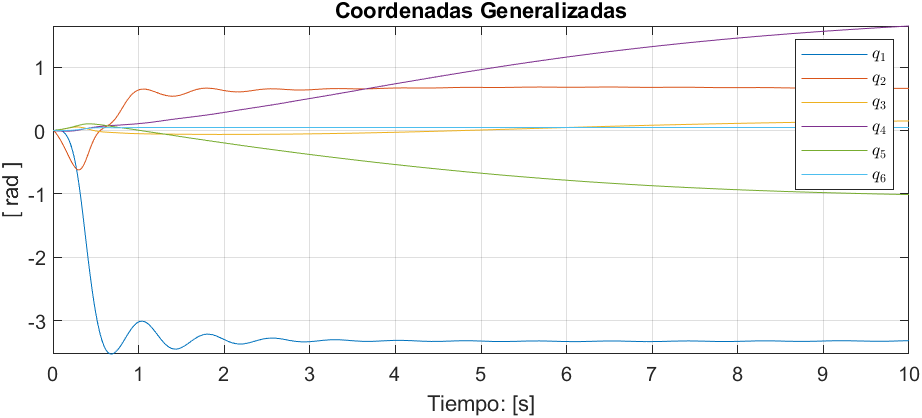
\includegraphics[scale=0.5]{coor_gen_caso_1.png} 
        \caption{Coordenadas Generalizadas Caso 1}
        \label{fig:CoordGenC1}
    \end{figure}

    \subsubsection{Velocidad Generalizada}
    La gráfica \ref{fig:VelGenC1}, presenta un cambio notable en la velocidad 
    de las articulaciones $q_1$ y $q_2$, esto debido a que ambas conforman 
    las articulaciones base del robot, y por lo tanto permiten definir la dirección 
    de movimiento del resto de los referenciales. De esta forma se explican las 
    variaciones de velocidad significativas de las primeras dos articulaciones, 
    mientras que el resto, cuyos eslabones se mueven en función de los dos primeros 
    en una respuesta libre del sistema, muestran variaciones menores de velocidad.

    \begin{figure}[H]% [!ht]
            \centering
            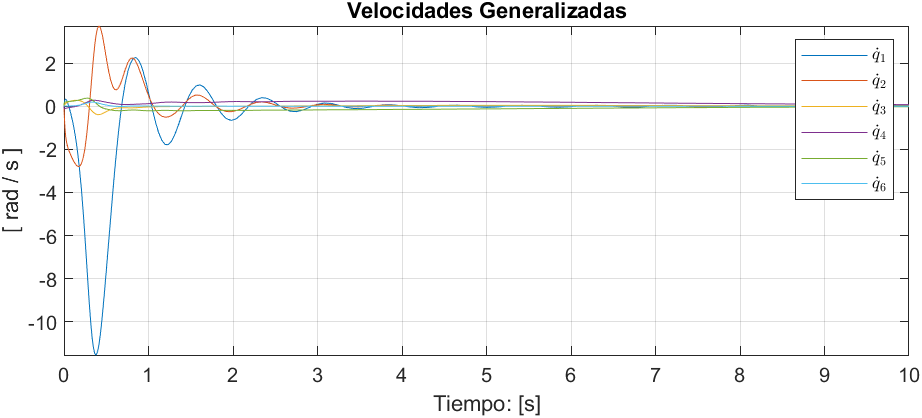
\includegraphics[scale=0.5]{vel_gen_caso_1.png} 
        \caption{Velocidad Generalizada Caso 1}
        \label{fig:VelGenC1}
    \end{figure}

    \subsubsection{Energía Cinética}

    En el caso de la figura \ref{fig:eCinC1} se identifica un pico en la energía 
    cinética a los 0.4 segundos y un punto de inflección hacia un estado estacionario 
    a partir del segundo 2, lo cual 
    es consistente con lo esperado, puesto que se observa una etapa de 
    amortiguamiento y pérdida de energía, hasta alcanzar el equilibrio. Esto significa 
    que cuando se suelta el exoesqueleto de su posición de \emph{Casa} y 
    empieze a moverse como un péndulo, llegará un instante en que se detenga el 
    movimiento oscilatorio, que es la fase de amortiguamiento observada.

    \begin{figure}[H]%[!ht]
            \centering
            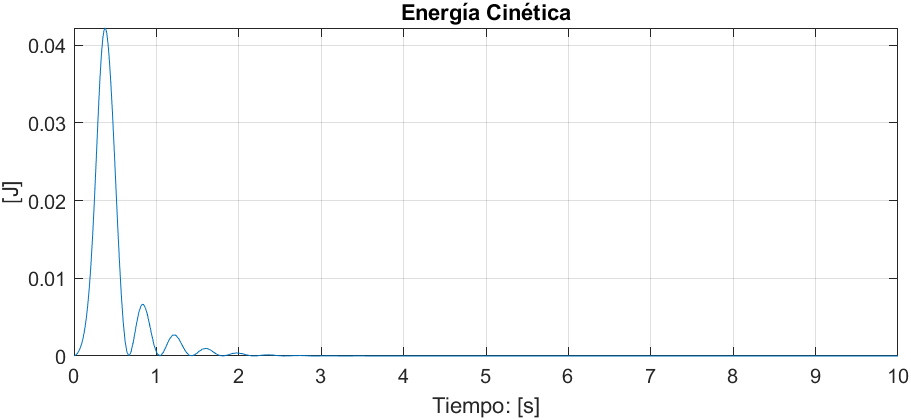
\includegraphics[scale=0.5]{ener_cin_caso_1.png} 
        \caption{Energía Cinética Caso 1}
        \label{fig:eCinC1}
    \end{figure}

    \subsubsection{Energía Potencial}
    La energía potencial inicia en 0.3 [J] y se puede observar en la figura 
    \ref{fig:ePotC1} que a partir del segundo 2 se llega a un punto de equilibrio al no tener 
    movimiento el exoesqueleto. Esto es consistente con los resultados obtenidos para 
    el rango máximo de la energía potencial, pues la misma o adquiere valores mayores al 
    inicial de la energía potencial, con lo cual se demuestra el efecto directo de las 
    fuerzas disipativas.

    \begin{figure} [H]%[!ht]
            \centering
            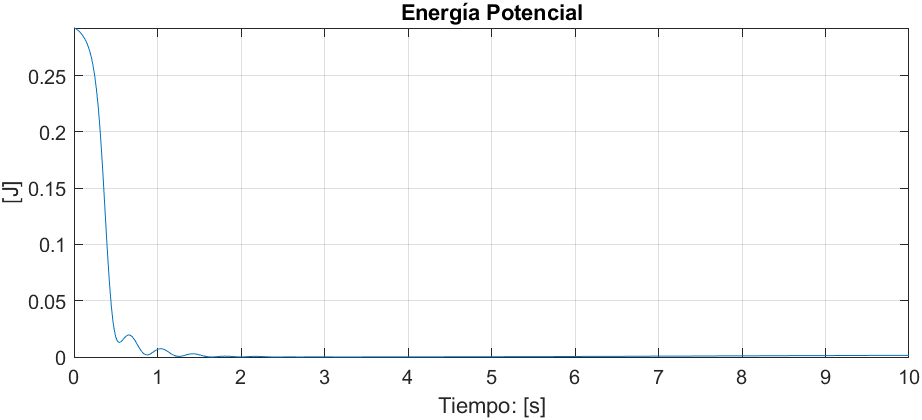
\includegraphics[scale=0.5]{ener_pot_caso_1.png} 
        \caption{Energía Potencial Caso 1}
        \label{fig:ePotC1}
    \end{figure}

    \subsubsection{Energía Mecánica}
    La energía mecánica es la suma de la energía cinética con la energía potencial. 
    la gráfica \ref{fig:eMecC1} resulta similar a la obtenida en \ref{fig:ePotC1} 
    debido a que la energía cinética presenta valores de una escala menor que los 
    obtenidos por la energía potencial, con lo cual es congruente que el comportamiento 
    del cambio de la energía mecánica dependa principalmente de este.

    \begin{figure} [H]%[!ht]
            \centering
            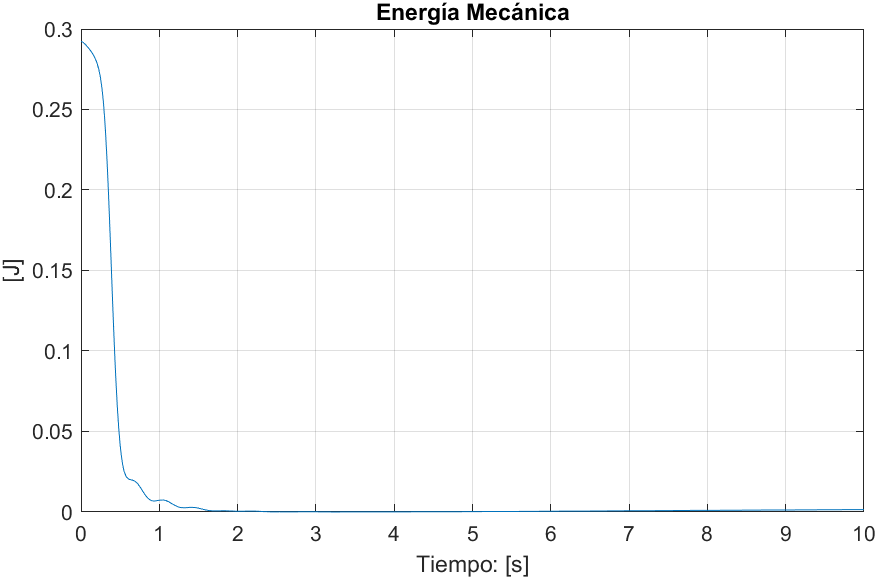
\includegraphics[scale=0.5]{ener_mec_caso_1.png} 
        \caption{Energía Mecánica Caso 1}
        \label{fig:eMecC1}
    \end{figure}

\subsection{Caso 2}\label{caso2}
    En el presente caso de estudio, se hicieron modificaciones en todos los 
    parámetros (torque, factor de disipación y tiempo de simulación), los 
    valores exactos se visualizan en la tabla \ref{ref:TablaC2}.

    \subsubsection{Parámetros} 
    \begin{table}[H]%[!ht]
        \centering
        \begin{center}
        \caption{Parámetros modificados del simulador (Sistema No Conservativo)} 
        \centering
        \bigskip
        \scalebox{0.7}{
            \begin{tabular}{c||cccccc|c}
            Parámetros & $\tau_1$ & $\tau_2$ & $\tau_3$ & $\tau_4$ & $\tau_5$ & $\tau_6$ & Unidades\\
            \hline
            Torques & -0.050 & 0.050 & -0.040 & -0.060 & 0.020 & 0.010 & [Nm] \\
            Factor de Disipación & \multicolumn{6}{c|}{0.006001} & [Ns/m] \\
            Tiempo de Simulación & \multicolumn{6}{c|}{20} & [s]\\
            \hline 
            \end{tabular}    }
        \end{center}
        \label{ref:TablaC2}
    \end{table}

    \subsubsection{Coordenadas Generalizadas}
    Las imágenes de la gráfica \ref{fig:CoordGenC2} son consistentes con los 
    valores dados en los torques, esto considerando que las fuerza aplicadas en las 
    articulaciones $q_1$, $q_3$ y $q_4$ se definieron con valores negativos,
    lo cual se ve representado en un giro en sentido negativo acorde a la regla 
    de la mano derecha.

    \begin{figure} [H]%[!ht]
            \centering
            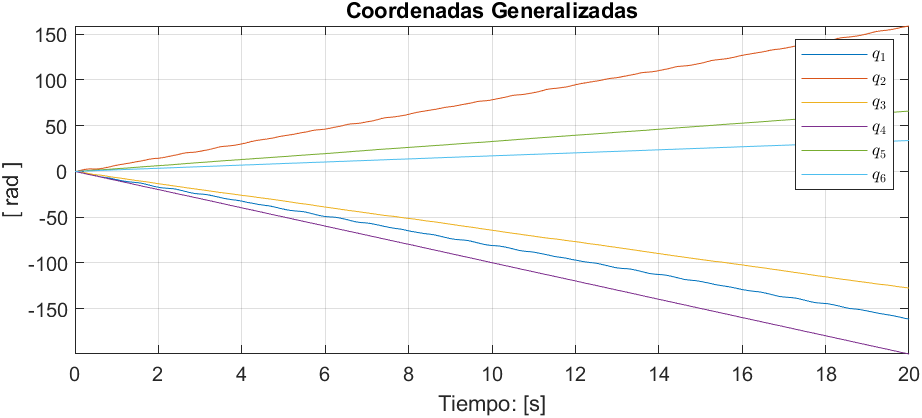
\includegraphics[scale=0.5]{coor_gen_caso_2.png} 
        \caption{Coordenadas Generalizadas Caso 2}
        \label{fig:CoordGenC2}
    \end{figure}

    \subsubsection{Velocidad Generalizada}
    Las articulaciones $q_1$ y $q_2$, en la gráfica \ref{fig:VelGenC2} 
    son las que presentan variaciones con una mayor amplitud de velocidad que el resto de 
    los valores de las velocidades generalizadas, 
    además se considera que las velocidades $\dot{q}_2$,$\dot{q}_5$ y 
    $\dot{q}_6$ toman valores positivos y esto es consistente con los torques aplicados.
    \begin{figure}[H]%[!ht]
            \centering
            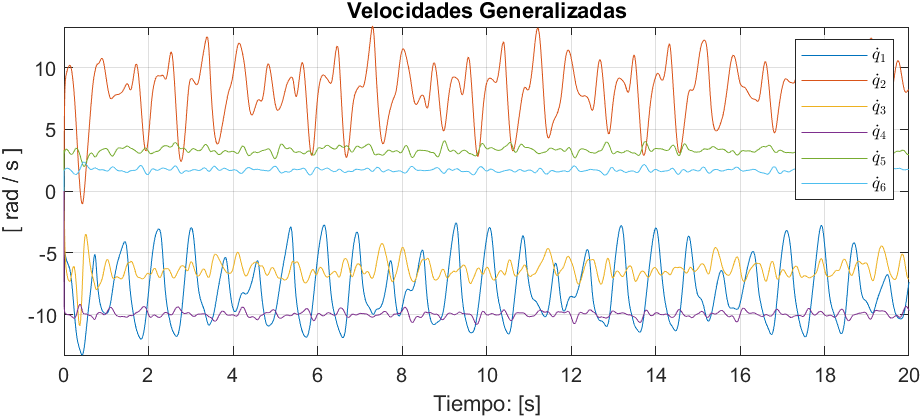
\includegraphics[scale=0.5]{vel_gen_caso_2.png} 
        \caption{Velocidad Generalizada Caso 2}
        \label{fig:VelGenC2}
    \end{figure}

    \subsubsection{Energía Cinética}
    La gráfica \ref{fig:eCinC2} demuestra una función periódica, la cual presenta valores 
    consistentes con el fenómeno físico que se observaría en el exoesqueleto al momento de 
    aplicar torques constantes, pues a diferencia del caso anterior en el que se presentaba 
    un punto de equilibrio, en este caso las articulaciones se encontrarían rotando de manera 
    permanente, con lo cual habría incrementos de energía cinética en todos los rangos en los que 
    se presente el giro en dirección al efecto de la fuerza de la gravedad, mientras que 
    la misma presentaría reducciones en el caso contrario.

    \begin{figure} [H]%[!ht]
            \centering
            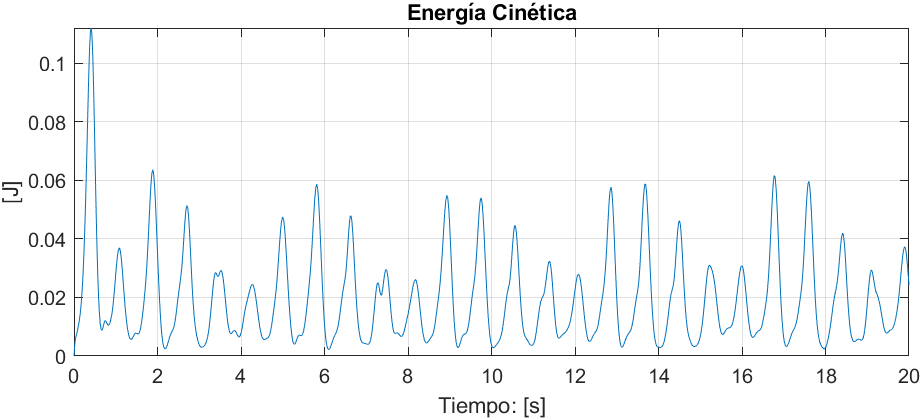
\includegraphics[scale=0.5]{ener_cin_caso_2.png} 
        \caption{Energía Cinética Caso 2}
        \label{fig:eCinC2}
    \end{figure}

    \subsubsection{Energía Potencial}
    La imagen obtenida por el osciloscopio, que se representa en la figura 
    \ref{fig:ePotC2}  muestra la periodicidad del movimiento que está teniendo 
    el exoesqueleto, algo importante a remarcar, es que está oscilando entre 
    los valores de 0[J] y 2.2[J], pero nunca llega a los mismos 3[J] de inicio, 
    debido a que posterior al estado base, el sistema no vuelve a tener todos 
    sus referenciales en la posición original. 
    
    Así mismo se observa que los puntos de energía potencial máxima, coinciden con 
    el inicio de los incrementos de energía cinética, con lo cual se refuerza la 
    idea del efecto de la fuerza de gravedad en relación a los incrementos y 
    decrementos de energía. 

    \begin{figure} [H]%[!ht]
            \centering
            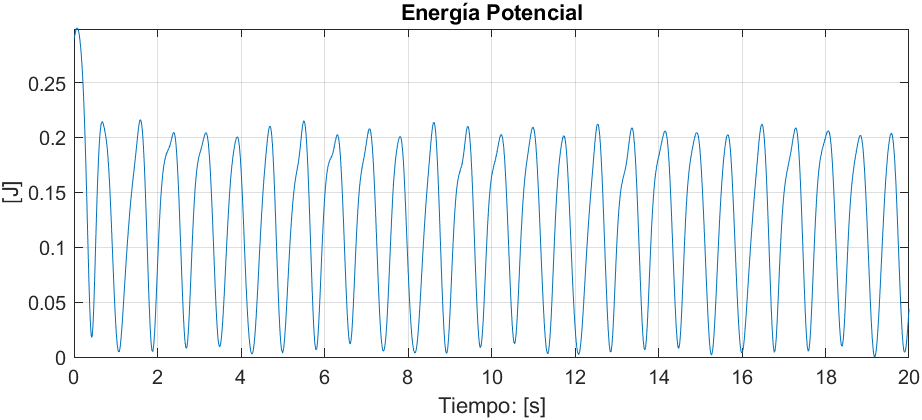
\includegraphics[scale=0.5]{ener_pot_caso_2.png} 
        \caption{Energía Potencial Caso 2}
        \label{fig:ePotC2}
    \end{figure}

    \subsubsection{Energía Mecánica}
    La gráfica de la figura \ref{fig:eMecC2} muestra un desfase positivo, 
    proporcional a la magnitud de la energía cinética, con respecto de la 
    gráfica de la figura \ref{fig:ePotC2}.
    \begin{figure} [H]%[!ht]
            \centering
            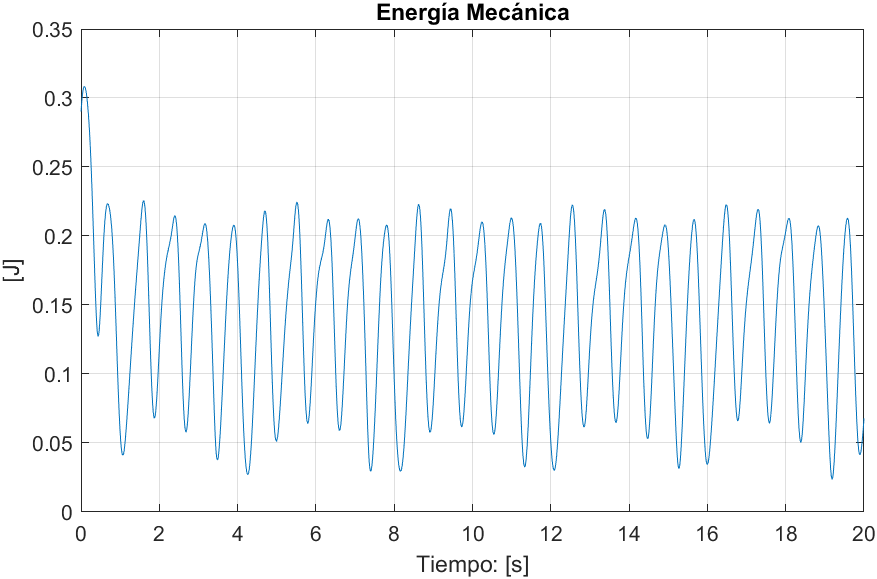
\includegraphics[scale=0.5]{ener_mec_caso_2.png} 
        \caption{Energía Mecánica Caso 2}
        \label{fig:eMecC2}
    \end{figure}

    

\subsection{Caso 3}\label{caso3}
    El último caso analizado representa un sistema conservativo, esto significa 
    un acercamiento a un sistema ideal donde no hay disipación de energía, 
    debido a que no se aplica una fuerza generada por una fricción viscosa.

    \subsubsection{Parámetros}

    Los parámetros que se utilizaron para el caso 3, se ven reflejados en la 
    tabla \ref{ref:TablaC3}, es decir, se están considerando torques nulos y 
    sin fricción, así mismo se incrementó el tiempo de simulación, para tener un 
    mayor espacio de muestreo en el análisis.

    \begin{table}[H]%[!ht]
        \centering
        \begin{center}
        \caption{Parámetros modificados del simulador (Sistema Conservativo)} 
        \centering
        \bigskip
        \scalebox{0.7}{
            \begin{tabular}{c||cccccc|c}
            Parámetros & $\tau_1$ & $\tau_2$ & $\tau_3$ & $\tau_4$ & $\tau_5$ & $\tau_6$ & Unidades\\
            \hline
            Torques & 0 & 0 & 0 & 0 & 0 & 0 & [Nm] \\
            Factor de Disipación & \multicolumn{6}{c|}{0} & [Ns/m] \\
            Tiempo de Simulación & \multicolumn{6}{c|}{200} & [s]\\
            \hline 
            \end{tabular}    }
        \end{center}
        \label{ref:TablaC3}
    \end{table}

    \subsubsection{Coordenadas Generalizadas}

    La gráfica \ref{fig:CoordGenC3} muestra los cambios en la posición 
    angular de cada una de las articulaciones a lo largo de 200 segundos 
    simulados, se aprecia que el 6to referencial $q_6$ es el que más rotaciones 
    presenta.

    \begin{figure} [H]% [!ht]
            \centering
            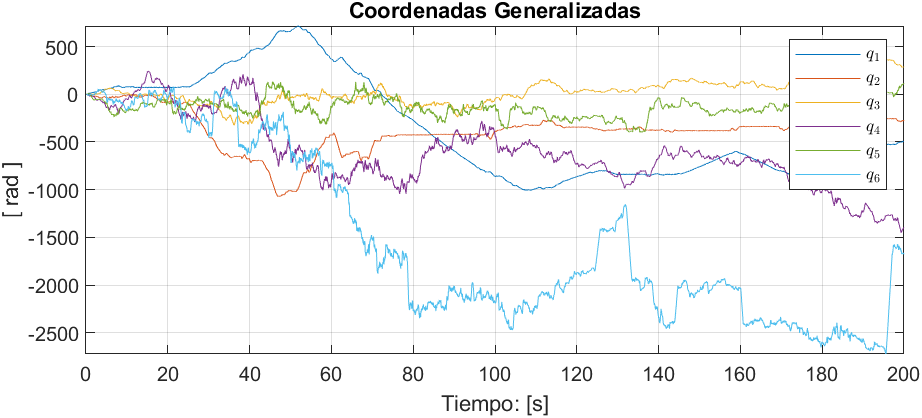
\includegraphics[scale=0.5]{coor_gen_caso_3.png} 
        \caption{Coordenadas Generalizadas Caso 3}
        \label{fig:CoordGenC3}
    \end{figure}

    \subsubsection{Velocidad Generalizada}

    La gráfica \ref{fig:VelGenC3} muestra en primer plano la velocidad 
    generalizada del referencial $q_6$ en azul claro, el cual en el espacio 
    de tiempo de 0 a 40 segundos presenta un incremento positivo en sus valores 
    absolutos de velocidad, alcanzando su punto máximo en el segundo 68, 
    a partir de ese momento empieza a disminuir su velocidad, para 
    finalmente estabilizar su valor en un rango de -1000 a 1000 
    rad/s, a partir de un tiempo de 120 segundos. 

    \begin{figure}[H]%[!ht]
            \centering
            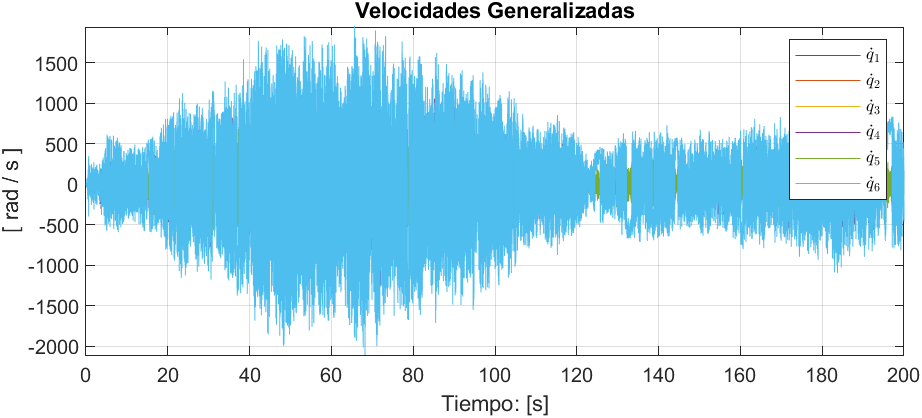
\includegraphics[scale=0.5]{vel_gen_caso_3.png} 
        \caption{Velocidad Generalizada Caso 3}
        \label{fig:VelGenC3}
    \end{figure}

    \subsubsection{Energía Cinética}

    La energía cinética representada en la gráfica \ref{fig:eCinC3} muestra 
    un pico a los 68 segundos, para finalmente tener un rango definido entre 
    0 y 1 Joule a partir de los 120 segundos.

    \begin{figure} [H]%[!ht]
            \centering
            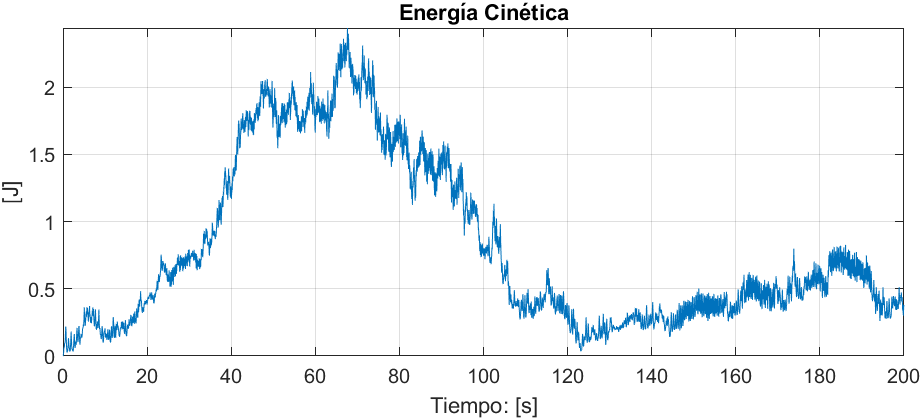
\includegraphics[scale=0.5]{ener_cin_caso_3.png} 
        \caption{Energía Cinética Caso 3}
        \label{fig:eCinC3}
    \end{figure}

    \subsubsection{Energía Potencial}

    La energía potencial es proporcional a la posición que tiene la cadena 
    cinemática en función a un "datum", debido a lo anterior la gráfica 
    \ref{fig:ePotC3} muestra que el exoesqueleto está tomando en promedio 
    valores constantes y cercanos a cero, por eso su rango está entre 0 y 
    0.3 [J], porqué está teniendo una rotación en un movimiento perpetuo, 
    al no haber fricción.

    \begin{figure} [H]%[!ht]
            \centering
            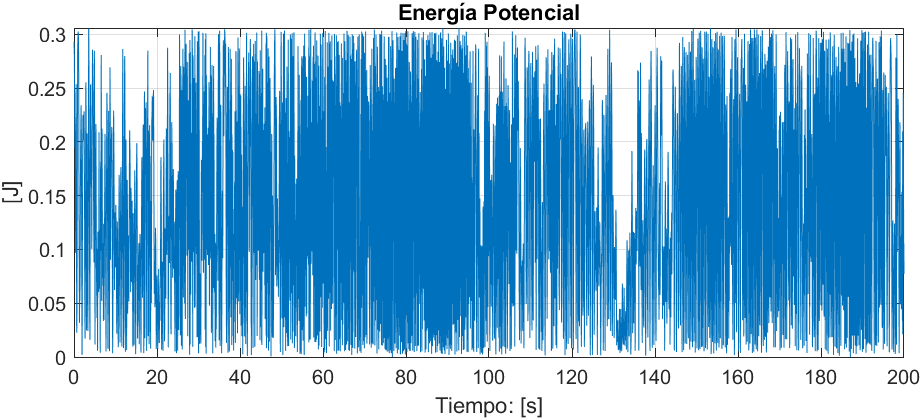
\includegraphics[scale=0.5]{ener_pot_caso_3.png} 
        \caption{Energía Potencial Caso 3}
        \label{fig:ePotC3}
    \end{figure}

    \subsubsection{Energía Mecánica}

    La gráfica \ref{fig:eMecC3} representa la energía mecánica total de 
    un sistema conservativo, cuyo valor máximo positivo es de 0.3 [J], puesto 
    que ese es el rango promedio máximo constante de la energía potencial. 
    El pico que se observa en el lapso del tiempo de 0 a 68 segundos 
    refleja una inconsistencia a las leyes de la termodinámica, debido 
    a que está reflejando creación de energía cinética, pues supera el 
    rango máximo de la energía potencial.

    \begin{figure}[H]%[!ht]
            \centering
            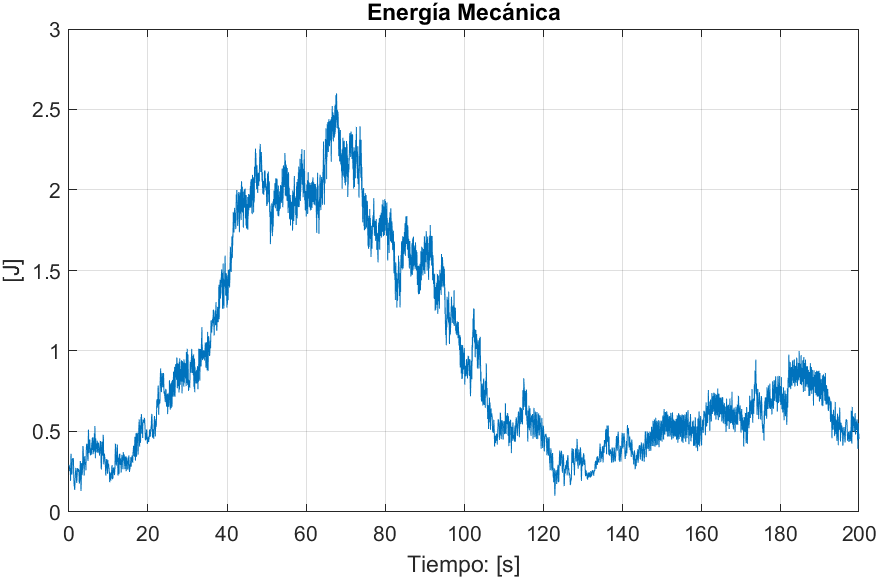
\includegraphics[scale=0.5]{ener_mec_caso_3.png} 
        \caption{Energía Mecánica Caso 3}
        \label{fig:eMecC3}
    \end{figure}

    \subsection{Análisis energético de sistema no conservativo}
    En la sección \ref{caso1}, se observa que el sistema se comporta de la manera 
    esperada ya  que al no existir la influencia de fuerzas exógenas $\boldsymbol{\tau}$ y considerando el efecto de las fuerzas 
    disipativas $\boldsymbol{\tau}_D$, se visualiza en la gráfica de energía mecánica una tendencia de la energía hacia cero, 
    indicando que toda la energía potencial presente en el estado inicial del robot se pierde conforme las articulaciones se mueven, 
    hasta llegar a un estado de reposo. 
    
    Considerando la sección \ref{caso2}, se observa que el sistema se comporta nuevamente como lo esperado, esto debido que 
    al aplicarse fuerzas exógenas $\boldsymbol{\tau}$ ocurre un aumento en la energía mecánica del sistema, transformándose así en 
    energía cinética para el movimiento de cada eslabón. 

    Esto además, permite definir que el torque aplicado a cada grado de libertad supera la fricción viscosa de la articulación, 
    haciendo que las coordenadas generalizadas $\boldsymbol{q}$ cambien de posición en función de la regla de la mano
    derecha.  

\subsection{Análisis energético de sistema conservativo}
    Si se realiza un análisis del caso de la sección \ref{caso3}, 
    se obtienen las Figuras \ref{fig:ec3} y \ref{fig:ep3}
    en un tiempo de $0$ a $5$ $[s]$ donde se representa el comportamiento 
    \emph{complementario} entre la energía cinética con la energía 
    potencial, con el fin de describir una energía mecánica constante. 
    
    \begin{figure}[H]
        \centering
        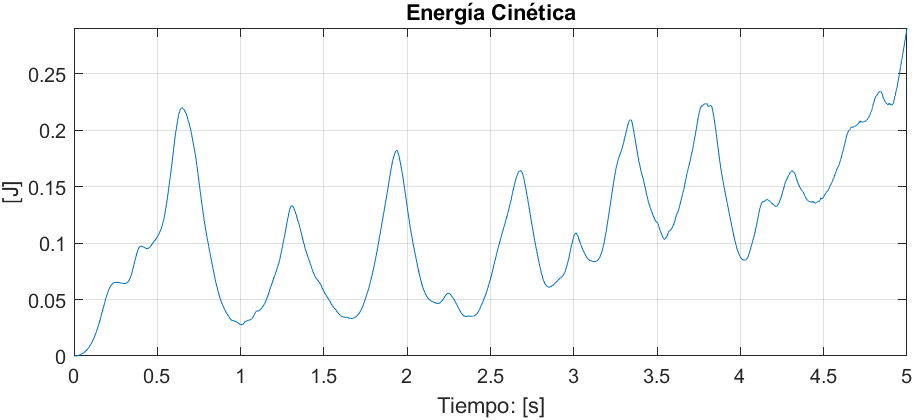
\includegraphics[scale=0.5]{Resultados/ener_cin_caso3_5s.png} 
        \caption{Energía cinética de caso 3, periodo de 5s.}
        \label{fig:ec3}
    \end{figure}

    \begin{figure}[H]
        \centering
        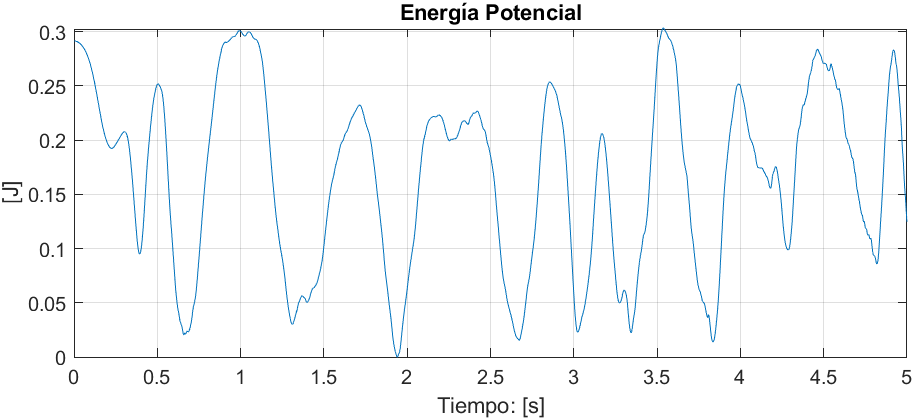
\includegraphics[scale=0.5]{Resultados/ener_pot_caso3_5s.png} 
        \caption{Energía potencial de caso 3, periodo de 5s.}
        \label{fig:ep3}
    \end{figure}

    Sin embargo, puede notarse un aumento en la energía cinética en los últimos segundos, 
    tal como se presenta en la Figura \ref{fig:eCinC3}. Esto es 
    incongruente con los resultados esperados dado que el sistema no puede tener mayor 
    energía cinética que la energía potencial máxima, puesto que no se aplica ninguna 
    fuerza exógena.

    % Punto 3
    Como tercer punto, asumiendo que los resultados incongruentes obtenidos para el 
    último caso de análisis energético son consecuencia del uso de un integrador 
    no adecuado para el tipo de sistema, se procedió a ejecutar el simulador 
    definiendo el integrador de paso fijo \emph{ode3} con un tamaño de paso de 
    0.00001s, esperando obtener una representación congruente con respecto a 
    la conservación de la energía.

    La gráfica de la energía mecánica resultante para un tiempo de $5[s]$ de simulación 
    se presenta en la figura \ref{fig:em_3_ode3}, y se observa que al compararse con la gráfica 
    de energía mecánica haciendo uso del integrador \emph{ode15s} en la figura \ref{fig:em_3}, ambas gráficas presentan 
    comportamientos similares, tanto en sus rangos de amplitud como en los valores que toman 
    en cada instante de tiempo.

    \begin{figure}[H]
        \centering
        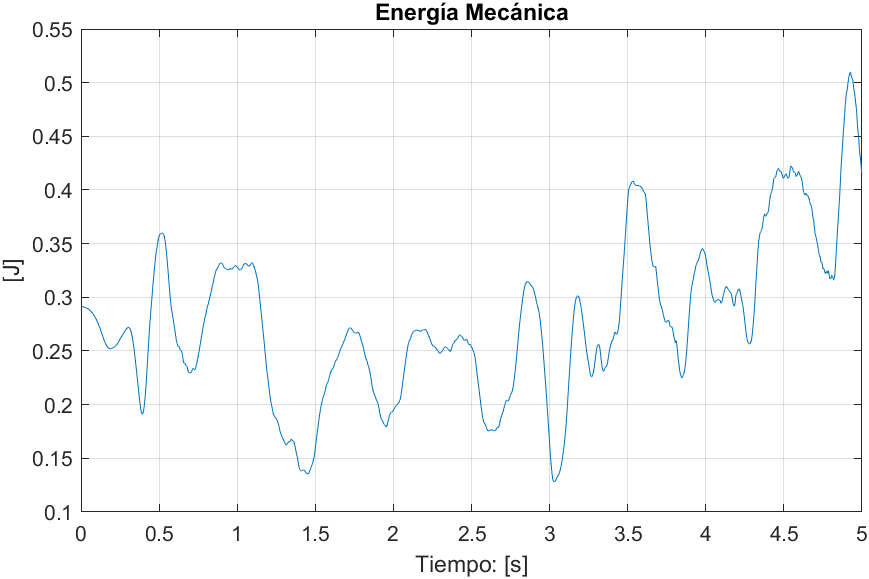
\includegraphics[scale=0.5]{Resultados/ener_mec_caso3_5s.png} 
        \caption{Energía mecánica de caso 3, periodo de 5s.}
        \label{fig:em_3}
    \end{figure}

    \begin{figure}[H]
        \centering
        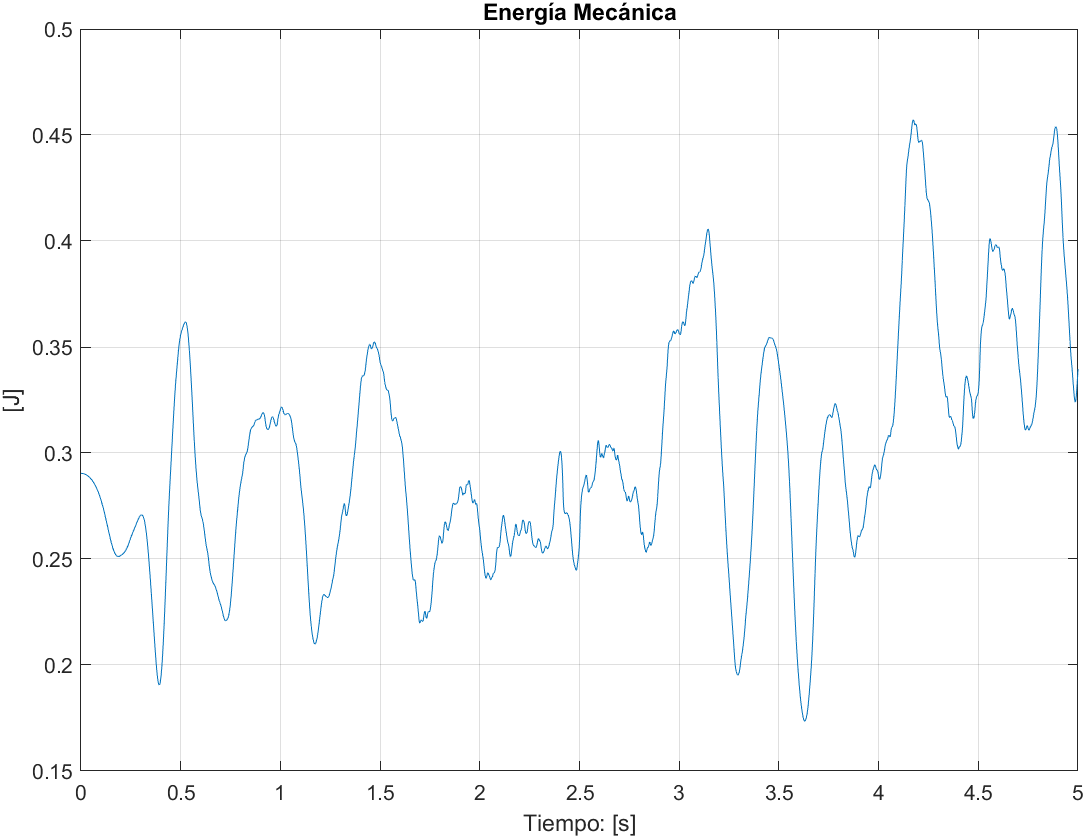
\includegraphics[scale=0.38]{Resultados/ener_mec_caso3_ode3_5s.png} 
        \caption{Energía mecánica de caso 3, periodo de 5s, integrador ode3.}
        \label{fig:em_3_ode3}
    \end{figure}

    De esta manera, se observa una diferencia entre los resultados obtenidos por cualquiera de los integradores con respecto a 
    los resultados esperados. Esta discrepancia puede atribuirse al hecho de que cualquier integrador basado 
    en métodos numéricos que dé solución al modelo dinámico, acumula un error si el tiempo de 
    muestreo utilizado no corresponde con la velocidad de la dinámica del sistema. Es decir, 
    considerando que las gráficas de velocidades generalizadas muestran que el eslabón asociado a $q_6$ 
    incrementa su velocidad en una escala mayor que la del resto de los eslabones, es posible 
    que la frecuencia de oscilación de dicho eslabón sea mayor que la frecuencia de muestreo del integrador 
    y por lo tanto, el causante del fallo en el proceso de integración.

\subsection{Trabajo futuro}
    Se contempla el desarrollo de un segundo simulador basado en 
    la teoría del Acercamiento de Descomposición de Cuerpos (BDA), con el 
    fin de comparar los resultados obtenidos por este simulador.
    
    El cambio de paradigma debería permitir mejorar los tiempos de ejecución, así 
    como reducir el error numérico, verificando si la causa del error para el caso 
    conservativo es debido a la naturaleza del integrador o por la estructura del 
    modelo dinámico actual.

    De igual manera, se analizará el comportamiento del sistema con diferentes métodos 
    de integración, con el objetivo de determinar el más adecuado. 





    \section{Conclusiones}

    \subsection{García Álvarez Gregorio Eliezer}
\noindent Se alcanzó el objetivo de este reporte  puesto que se efectuó el simulador dinámico, así como su comportamiento
semejante a lo esperado en la realidad, en el caso del sistema no conservativo.
En el caso del sistema sin considerar la fricción viscosa, se obtuvieron resultados no esperados que se analizaron
y discutieron a profundidad, con el objetivo de identificar el error para poder implementar una solución adecuada. 
Se concluye que la discrepancia es debida al integrador. 

Una hipótesis es la siguiente:
Debido a que sobre el sistema solo actúa la fuerza de gravedad, al soltarse el exoesqueleto de su posición vertical
de "casa", se empieza a acelerar y a partir del segundo 5 aún no alcanza una velocidad constante porque el sistema
se puede considerar como un péndulo compuesto de 7 eslabones, lo que conlleva a un sistema caótico (sin embargo
continúa siendo determinista). Es importante remarcar que el 6to referencial presenta una velocidad mayor al del
resto de los eslabones, porque al ser tan pequeño en relación a los demás, implica que tiene el menor momento de
inercia. Al ser el último eslabón el que mayor velocidad tiene, este influye considerablemente en la trayectoria de
la cadena cinemática. Y estos cambios de aceleraciones sobrepasan al tiempo de procesamiento del integrador, 
acumulando un error numérico y mostrando datos imposibles (crear energía).

Por otro lado, un simulador tiene como objetivo experimentar en un entorno virtual, así como ayudar a comprobar
hipótesis. Un ejercicio que se me ocurrió, puede ser el de ejemplificar la teoría del caos, en el caso de un sistema
no conservativo y ceros torques, debido a que el exoesqueleto en estas condiciones se comporta como un péndulo
compuesto. Finalmente, en la animación y las gráficas de posiciones generalizadas del caso 2, observé un cambio de 
giro; esto lo atribuyo al teorema del eje intermedio, sin embargo con los actuales datos no puedo asegurar que este
sucediendo esto, en este momento solo me limito a una interpretación de las gráficas y de lo visualizado en la
animación.
    
    \subsection{Luna Macías Antonio de Jesús}
    \blindtext[0]
    \subsection{Tevera Ruiz Alejandro}
\blindtext[0]

    \section{Anexos}
\blindtext[0]
\blindtext[0]
\blindtext[0]

\end{document}